\centering
\def\distance{0.0cm}
\def\distancePlotLabel{8.5cm}
\def\heightplots{2.2cm}
\begin{tikzpicture}[thick]

%%%%%%%%%%%%%%%%%%%%%%%%%%%%%%%%%%%%%%%%%%%%%%%%%%%%%%%%%%%%
%%%%%%%%%%%%  Code             %%%%%%%%%%%%%%%%%%%%%%%%%%%%%
%%%%%%%%%%%%%%%%%%%%%%%%%%%%%%%%%%%%%%%%%%%%%%%%%%%%%%%%%%%%

  %%%%%%%%%%%%%%%%%%%
  %%%%%  Nodes  %%%%%
  %%%%%%%%%%%%%%%%%%%
  % (b)
  \node (b_code){
  \tiny\begin{lstlisting}[mathescape, escapeinside={(*@}{@*)}]
assume f = (x) -> {exp(-0.1 * abs(x - 2)) * 10 * cos(0.4 * x ) + 0.2};(*@\vspace{1mm}@*)
define x_prime = linspace(-20,20,200);(*@\vspace{1mm}@*)
define plot_curve_gp_predictive = ( ) -> {
  action(line_plot(x_prime, run(sample(f_emulate[1]((*@\$@*){x_prime}))), dict("color", "green")))};
  \end{lstlisting}
  };

  %%%%%%%%%%%%%%%%%%%
  %%%%%  Labels  %%%%
  %%%%%%%%%%%%%%%%%%%
  %\node[above=1 cm of start] (alabel) {(a) \gpmem: Schematic};
  \node[left=0.0cm of b_code] (b) {(b)};
  \node[above=3.0cm of b] (a) {(a)};
  \node[below=1.4cm of b] (c) {(c)};
  \node[below=1.8cm of c] (d) {(d)};
  \node[below=1.7cm of d] (e) {(e)};
  \node[below=1.8cm of e] (f) {(f)};
  \node[below=1.7cm of f] (g) {(g)};

  % (c)
  \node[right=\distance of c,yshift=0.1cm] (c_code){
  \tiny\begin{lstlisting}[mathescape, escapeinside={(*@}{@*)}]
assume scale_factor $\sim$ gamma(1,1); 
assume lengthscale $\sim$ uniform_continuous(0,10);  
assume zero_mean_function = gp_mean_const(0);
assume kse = gp_cov_scale(scale_factor, gp_cov_se(lengthscale));
assume (f_emulate, f_compute) = gpmem(f, zero_mean_function, kse);(*@\vspace{1mm}@*)
repeat(50, {plot_curve_gp_predictive()});
line_plot(x_prime,
  run(sample(mapv(f, (*@\$@*){x_prime}))),
  dict("color", "blue"));
  \end{lstlisting}
  };
  % (d)
  \node[right=\distance of d,yshift=0.1cm] (d_code){
  \tiny\begin{lstlisting}[mathescape, escapeinside={(*@}{@*)}]
predict f_compute(12.6);(*@\vspace{1mm}@*)
repeat(50, {plot_curve_gp_predictive()});
line_plot(x_prime,
  run(sample(mapv(f, (*@\$@*){x_prime}))),
  dict("color", "blue"));
  \end{lstlisting}
  };


  % (e)
  \node[right=\distance of e,yshift=0.1cm] (e_code){
  \tiny\begin{lstlisting}[mathescape, escapeinside={(*@}{@*)}]
predict f_compute(-6.4);(*@\vspace{1mm}@*)
repeat(50, {plot_curve_gp_predictive()});
line_plot(x_prime,
  run(sample(mapv(f, (*@\$@*){x_prime}))),
  dict("color", "blue"));
  \end{lstlisting}
  };


  % (f)
  \node[right=\distance of f,yshift=0.1cm] (f_code){
  \tiny\begin{lstlisting}[mathescape, escapeinside={(*@}{@*)}]
observe f_emu(-3.1) =  2.15;
observe f_emu(7.8)  = -5.40;
observe f_emu(0.0)  = 8.39;(*@\vspace{1mm}@*)
repeat(50, {plot_curve_gp_predictive()});
line_plot(x_prime,
  run(sample(mapv(f, (*@\$@*){x_prime}))),
  dict("color", "blue"));
  \end{lstlisting}
  };
  % (g)
  \node[right=\distance of g,yshift=0.1cm] (g_code){
  \tiny\begin{lstlisting}[mathescape, escapeinside={(*@}{@*)}]
mh(minimal_subproblem(random_singleton(/*)), 50);(*@\vspace{1mm}@*)
repeat(50, {plot_curve_gp_predictive()});
line_plot(x_prime,
  run(sample(mapv(f, (*@\$@*){x_prime}))),
  dict("color", "blue"));
  \end{lstlisting}
  };



  % samples/curve images
  \node[right=\distancePlotLabel of c, yshift=0.0] (c_pic){
  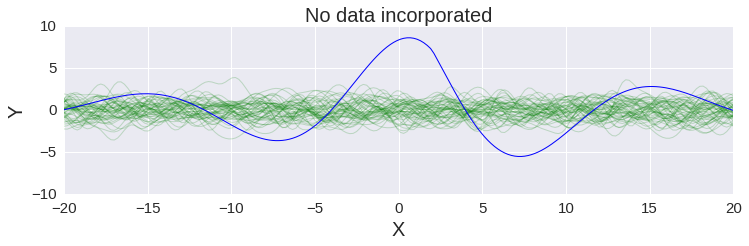
\includegraphics[height=\heightplots]{figs/revised_figures/tutorial_1.png}
  };
  \node[right=\distancePlotLabel of d, yshift=0.0] (d_pic){
  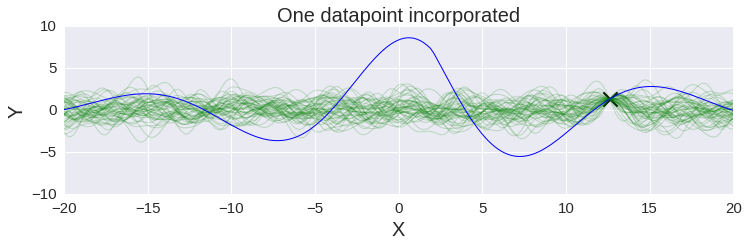
\includegraphics[height=\heightplots]{figs/revised_figures/tutorial_2.png}
  };
  \node[right=\distancePlotLabel of e, yshift=0.0] (e_pic){
  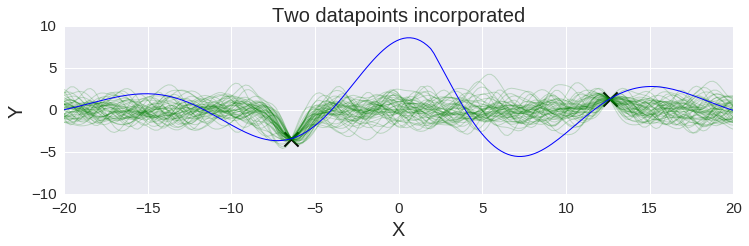
\includegraphics[height=\heightplots]{figs/revised_figures/tutorial_3.png}
  };
  \node[right=\distancePlotLabel of f, yshift=0.0] (f_pic){
  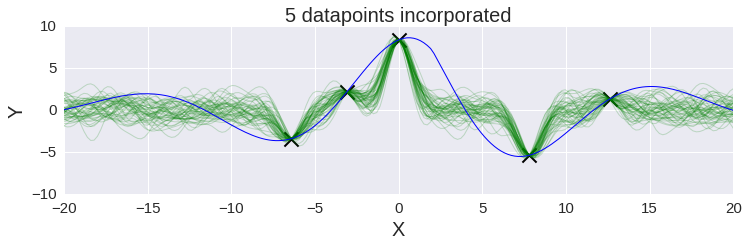
\includegraphics[height=\heightplots]{figs/revised_figures/tutorial_4.png}
  };
  \node[right=\distancePlotLabel of g, yshift=0.0] (g_pic){
  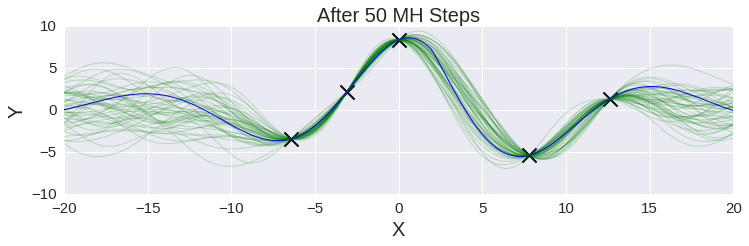
\includegraphics[height=\heightplots]{figs/revised_figures/tutorial_5.png}
  };


  % horizontal lines
  \node[right=0.0cm of b] (first_line_start){};
  \node[right=15.0cm of b] (first_line_end){};
  \node[below=0.2cm of b_code.north] (helper){};
  \draw 
    (first_line_start |- helper) -- (first_line_end |-  helper); 
  \draw 
    (first_line_start |-  b_code.south west) -- (first_line_end |- b_code.south east);   
  \draw 
    (first_line_start |- c_pic.south west) -- (first_line_end |- c_pic.south east);   
  \draw 
    (first_line_start |- d_pic.south west) -- (first_line_end |- d_pic.south east);   
  \draw 
    (first_line_start |- e_pic.south west) -- (first_line_end |- e_pic.south east);   
  \draw 
    (first_line_start |- f_pic.south west) -- (first_line_end |- f_pic.south east);   
  %% arrows
  %% (d)
  %\node[below = -2.45cm of d_pic,xshift=1.53cm] (arrow_d_end){};
  %\node[below = -1.45cm of d_pic,xshift=1.53cm] (arrow_d_head){};
  %\draw[green,->] (arrow_d_end) -- (arrow_d_head);
  %% (e)
  %\node[below = -1.9cm of e_pic,xshift=-0.62cm] (arrow_e_end){};
  %\node[below = -0.9cm of e_pic,xshift=-0.62cm] (arrow_e_head){};
  %\draw[green,->] (arrow_e_end) -- (arrow_e_head);
  %% (f)
  %\node[below = -2.49cm of f_pic,xshift=-0.26cm] (arrow_f_end1){};
  %\node[below = -1.49cm of f_pic,xshift=-0.26cm] (arrow_f_head1){};
  %\draw[->] (arrow_f_end1) -- (arrow_f_head1);
  %\node[below = -2.05cm of f_pic,xshift=0.1cm] (arrow_f_end2){};
  %\node[below = -1.05cm of f_pic,xshift=0.1cm] (arrow_f_head2){};
  %\draw[->] (arrow_f_head2) -- (arrow_f_end2);
  %\node[below = -2.45cm of f_pic,xshift=1.53cm] (arrow_f_end3){};
  %\node[below = -1.45cm of f_pic,xshift=1.53cm] (arrow_f_head3){};
  %\draw[->] (arrow_f_end3) -- (arrow_f_head3);


%%%%%%%%%%%%%%%%%%%%%%%%%%%%%%%%%%%%%%%%%%%%%%%%%%%%%%%%%%%%
%%%%%%%%%%%%%%%%%       Schematic       %%%%%%%%%%%%%%%%%%%%
%%%%%%%%%%%%%%%%%%%%%%%%%%%%%%%%%%%%%%%%%%%%%%%%%%%%%%%%%%%%

  %%%%%%%%%%%%%%%%%%%
  %%%%%  Nodes  %%%%%
  %%%%%%%%%%%%%%%%%%%
  
  \node[above=5.6cm of b, xshift = 8cm] (start) {};


  \node[draw,circle,minimum size=1.5cm,left = 0.5cm of start] (f) {f$_{\text{compute}}$};


  \node[draw,right = 0.5cm of start,circle,minimum size=1.5cm] (K) {$\kse \midtheta$};


  \node[draw,rectangle,below=1.2cm of start, text width = 8cm] (gpmem){
    \centering \texttt{gpmem}\vspace{0.2mm}

    \small$\text{memo table} = (\xbf,\ybf)$\vspace{0.2mm}

    \small$\;\;\;\;\;\;\;\;\;\;P(f_{emu}(x) \mid \xbf,\ybf,\thetabf)\sim
    \mathcal{N}\big(\mupost,\Kpost)\big)$

    };


  \node[draw,rectangle,dashed,right=1.6cm of K, text width = 3.4cm] (math){
    \footnotesize $\kse\,= \sigma^2 \exp(-\frac{(x-x^\prime)^2}{2\ell^2})$\vspace{1mm}

    $\thetabf \;\;\,\,= \{\sigma,\ell \} \rightarrow$ Scope\vspace{1mm}

    $\sigma\;\;\; \sim P(\sigma)\,$\vspace{1mm}

    $\ell\;\;\;\, \sim P(\ell)\;\,$\vspace{1mm}

   };


  \node[draw,rectangle,dashed,minimum size=1cm,left= 2.2cm of f] (resources){
    
\includegraphics[width=2.8cm]{figs/resources.jpg}};


  \node[draw,rectangle,below=0.8cm of gpmem,text width =7cm] (f_emu){
    \centering $f_{emu}$ \vspace{1mm}

    \renewcommand{\arraystretch}{0.5}
    \begin{tabular}{l|l}\footnotesize
       \footnotesize$x$ & \footnotesize$f(x)$ \\ \hline
       \footnotesize $x_1$  &\footnotesize$y_1$ \\
       \footnotesize  $x_2$  & \footnotesize$y_2$ \\
       \footnotesize$\cdots$ & \footnotesize $\cdots$
    \end{tabular}
    $\;\;\;\;$
    \begin{tabular}{l}
      \small Parameters:\\
      \small  Kernel lengthscale $\ell$  \\
      \small Kernel scale-factor $sf$
     \end{tabular}
  };


  \node[below =.1ex of gpmem,inner sep = 0pt,outer sep=0pt,xshift=-0.3cm] (helper1){};


  \node[below =.1ex of gpmem,inner sep = 0pt,outer sep=0pt,xshift=0.7cm] (helper2){};


  \node[above =.1ex of f_emu,inner sep = 0pt,outer sep=0pt, xshift=0mm] (helper_emu){};


  \node[above = 0.75cm of resources,inner sep = 0pt,outer sep=0pt] (helper_resource_top){};


  \node[left = 1cm of f_emu] (x_hat){$\xprime$} ;


  \node[right = 1cm of f_emu] (GaussianHat){$\yprime$} ;



  %%%%%%%%%%%%%%%%%%%
  %%%%% Arrows  %%%%%
  %%%%%%%%%%%%%%%%%%%

  \draw[thick,dashed,->] (resources) --node [pos=0.5,below] {\footnotesize resource}  node [pos=0.5,above] {\footnotesize outside} (f);

  \draw[thick,dashed,->] (math) -- node [pos=0.5,above] {\footnotesize Kernel} (K);

  \draw[thick,->] (K) -- (gpmem);

  \draw[thick,->] (f) -- (gpmem);

  \draw[thick,->] (gpmem) -- (f_emu);

  \draw[thick,->,dashed] (x_hat) -- (f_emu);

  \draw[thick,->,dashed] (f_emu) -- (GaussianHat);

\end{tikzpicture}

